\documentclass{standalone}
\standaloneconfig{border=2mm 2mm 2mm 2mm}


%maths
\usepackage{mathtools}
\usepackage{amsmath}
\usepackage{amssymb}
\usepackage{amsfonts}

%tikzpicture
\usepackage{tikz}
\usepackage{scalerel}
\usepackage{pict2e}
\usepackage{tkz-euclide}
\usetikzlibrary{calc}
\usetikzlibrary{patterns,arrows.meta}
\usetikzlibrary{shadows}
\usetikzlibrary{external}

%pgfplots
\usepackage{pgfplots}
\pgfplotsset{compat=newest}
\usepgfplotslibrary{statistics}
\usepgfplotslibrary{fillbetween}

%colours
\usepackage{xcolor}

\usepackage{nicefrac}

\begin{document}
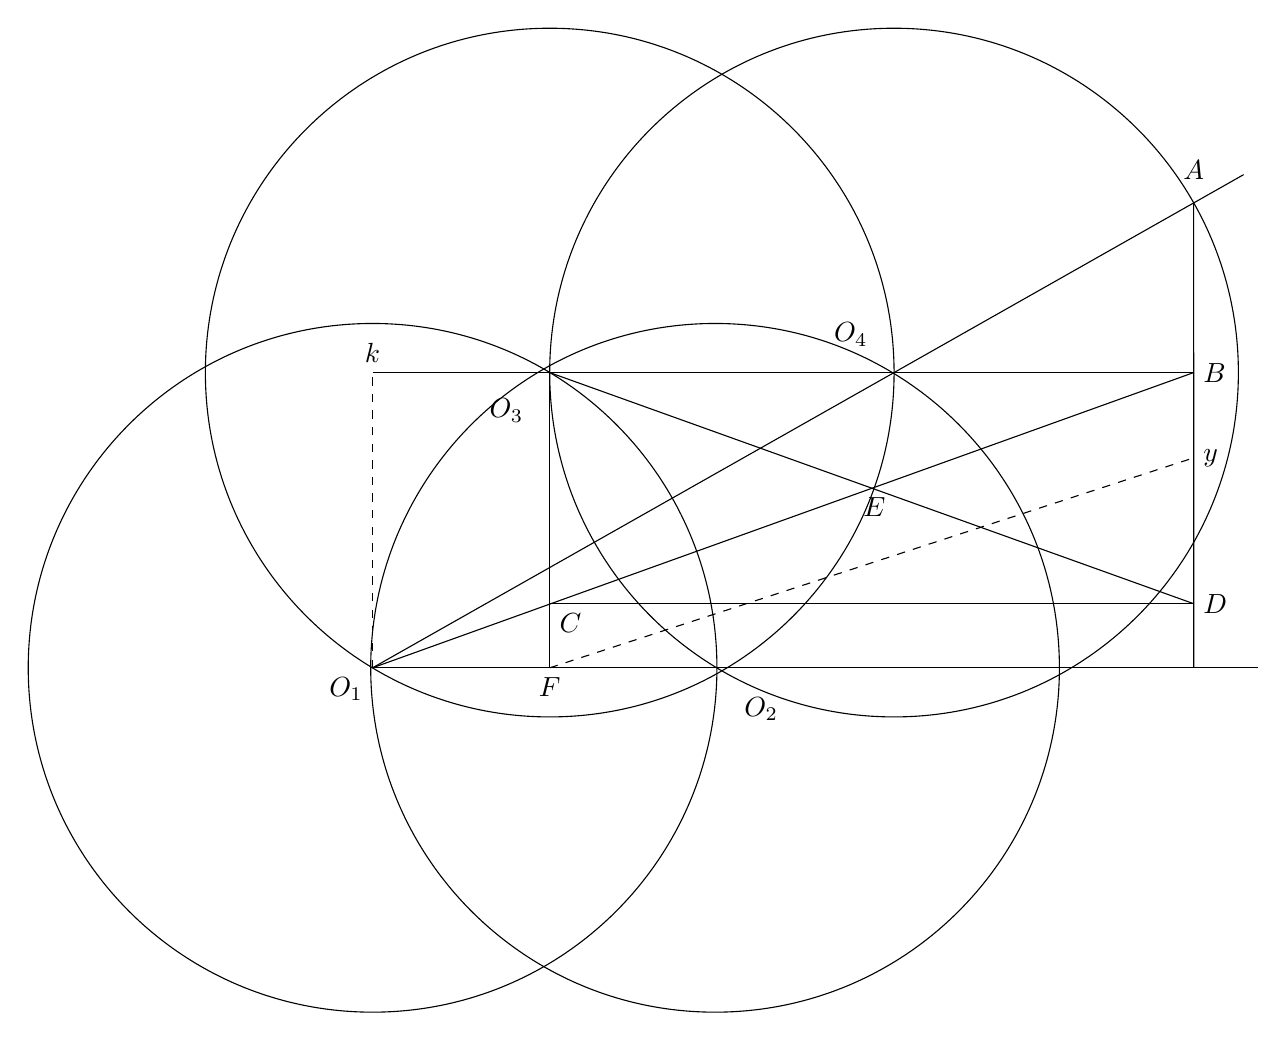
\begin{tikzpicture}[scale=1.5]

\coordinate[label=below left:{$O_1$}] (O_1) at (1, 0);
\coordinate[label=above:{$k$}] (k) at (1, 2.5);
\coordinate (O_3) at (2.5, 2.5);
\coordinate[label=below:{$F$}] (F) at (2.5, 0);
\coordinate (O_4) at (5.4154759474227, 2.5);
\coordinate (O_2) at (3.9, 0);
\coordinate (A) at (7.9525228450119, 3.9364515444083);
\coordinate[label=right:{$B$}] (B) at (7.9525228450119, 2.5);
\coordinate[label=right:{$D$}] (D) at (7.9525228450119, 0.5428891353198);
\coordinate[label=below right:{$C$}] (C) at (2.5, 0.5428891353198);
\coordinate[label=right:{$y$}] (R) at (7.9525228450119, 1.7779076795793);
\coordinate[label=below:{$E$}] (E) at (5.248515604993, 1.527548474);

\draw (O_1) circle [radius=2.9154759474227];
\draw (O_2) circle [radius=2.9154759474227] node[below right=10pt] {$O_2$};
\draw (O_3) circle [radius=2.9154759474227] node[below left=0.3cm] {$O_3$};
\draw (O_4) circle [radius=2.9154759474227] node[above left=0.3cm] {$O_4$};
\draw[dashed] (O_1)--(k);
\draw (k)--(B);
\draw (O_1)--(8.5, 0);
\draw (F)--(O_3);
\draw (O_1)--(8.374737697629, 4.175505531);
\draw (7.9525228450119, 0) -- (A) node[above=5pt] {$A$};
\draw (O_1)--(B);
\draw (C)--(D);
\draw (O_3)--(D);
\draw[dashed] (F)--(R);

\end{tikzpicture}
\end{document}
